
\section{Experiment description}\label{experiment-description}

\subsection{General perspective}\label{general-perspective}

Figure \ref{fig:experiment-overall-layout} shows default experiment layout. We have 3 laptops: two \glspl{ap} and one \glspl{command_n_center}. \Gls{command_n_center} use external \gls{wifi} adapter to set up wireless point for \glspl{ap} to access provided services. Each \acrshort{access_point} has two \gls{wifi} adapters: one used to set up \gls{wifi} access point for \glspl{ue}, the second (internal, built in the vast majority of modern laptops) adapter is used for connection to \gls{command_n_center}.

\begin{figure}[H]
\centering
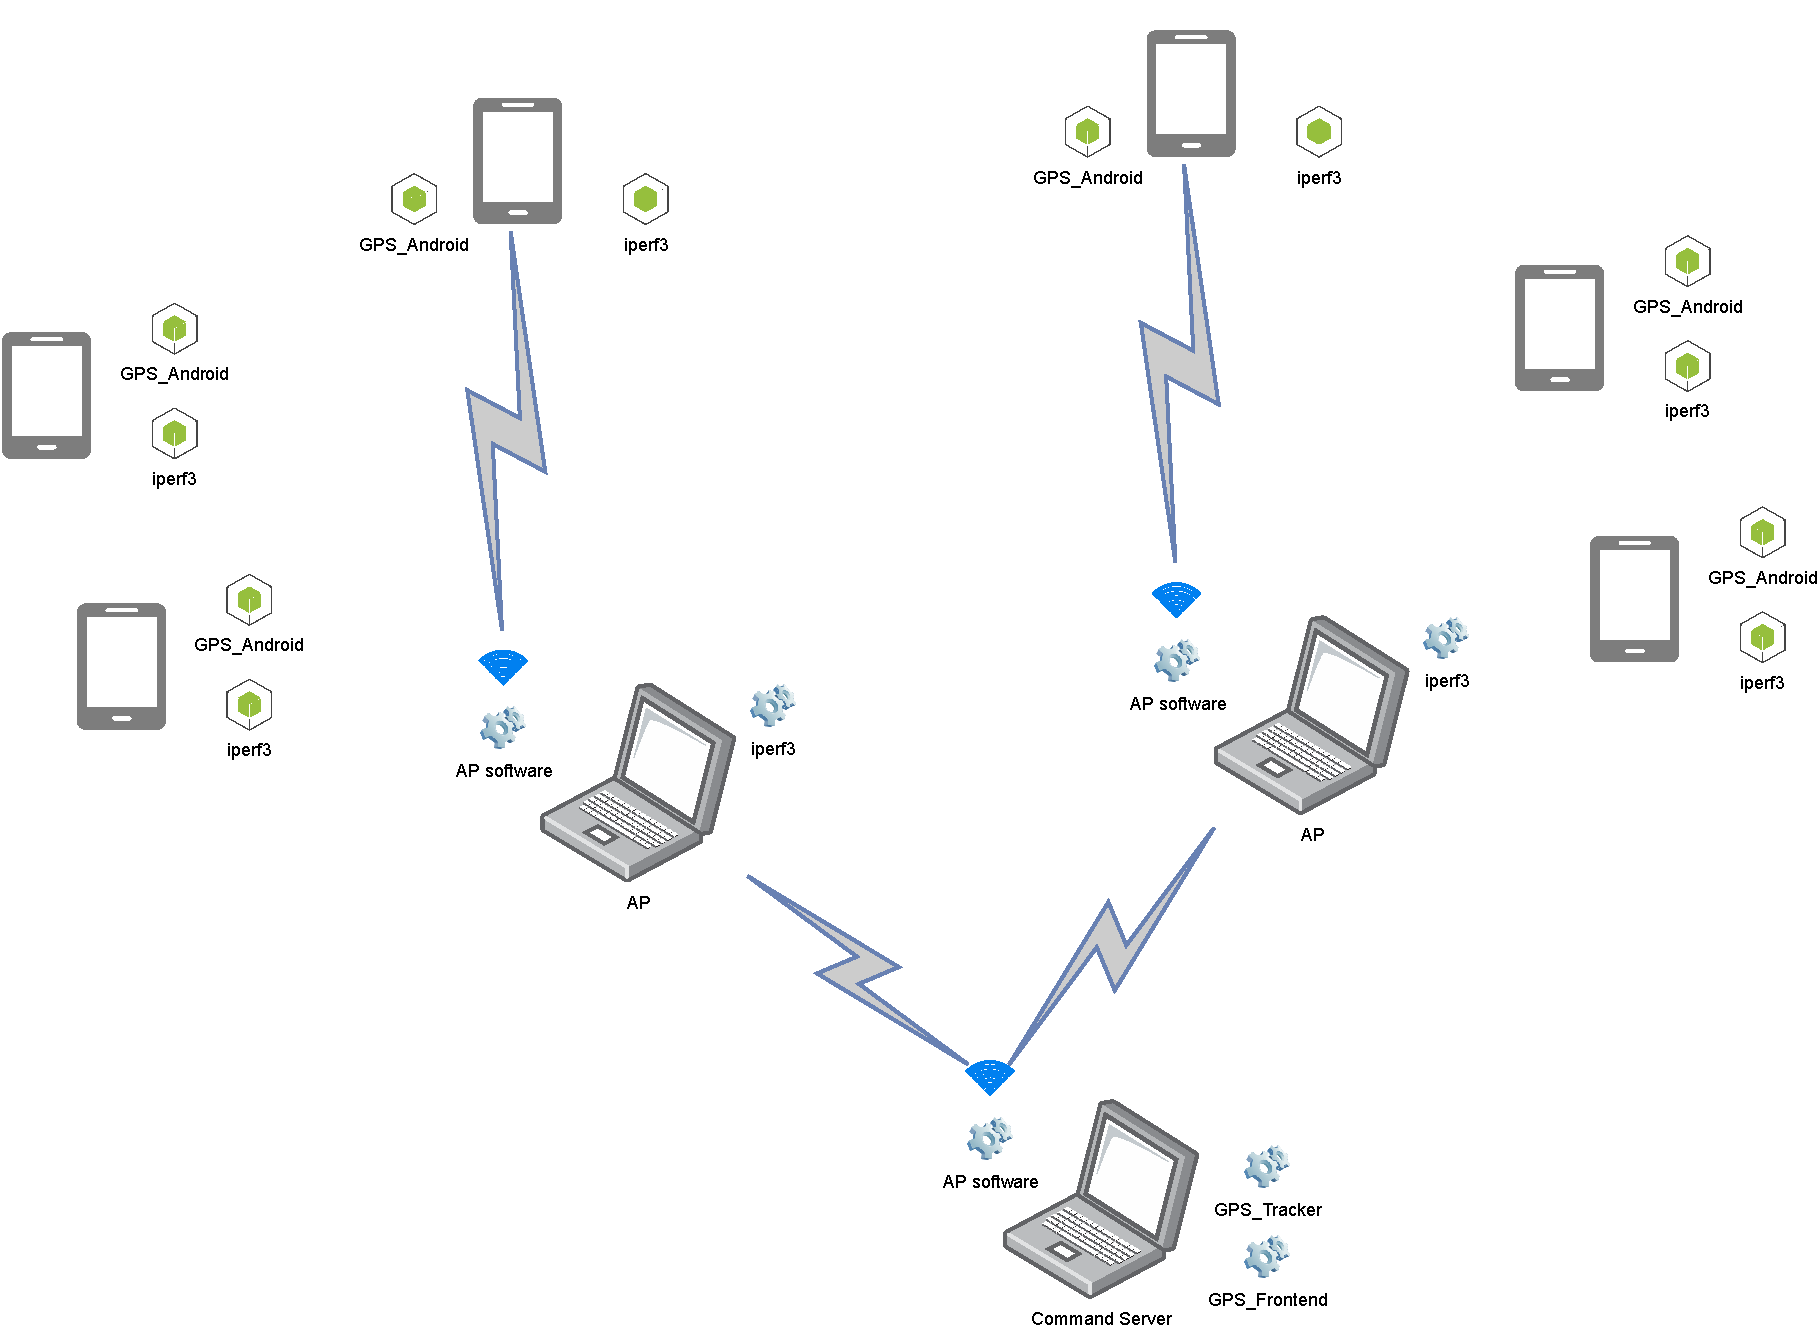
\includegraphics[width=\linewidth,keepaspectratio]{images/Deployment Diagram-Free-structure_scheme.pdf}
\caption{Main scenario of the experiment}
\label{fig:experiment-overall-layout}
\end{figure}

From the general system engineering perspective, the experiment is a set
of wireless-connected nodes (via \gls{wifi} 802.11n (300 mbps)) which measures the receiving signal strength and measure the throughput of the link to upload and download.

Preliminary tests in default layout showed one restrictions on experiment activity: network bandwidth
between \gls{ue} and \acrshort{access_point} measurements with \texttt{iperf3} showed about \textbf{30 MBit/s} speed rate. On the contrary, speed on the bearer \gls{ue} - \acrshort{access_point} - \gls{command_n_center} showed about \textbf{12-15 MBit/s} speed rate. This is significant drop in network rate, probably, because of transmission on the radio channel two-times. The problem  is not in the \gls{wifi} itself, but in the fact that radio (wireless) link is not as reliable compared to a wired one, so the active bandwidth measurement part must be located close to the \glspl{ap},thus \acrshort{ftp}-server placed in \gls{ap}.

Each \gls{ue} has   \gls{gps_android} installed. \Gls{access_point} create a \gls{wifi} access point named ``\textbf{ap}''.
\Gls{command_n_center} runs a wireless point named
``\textbf{cnc}''.

\subsection{Deployment diagram}\label{deployment-diagram}

Figure \ref{fig:deployment-diagram} shows components and their communication in the deployed phase. Each building block has certain level of independence, therefore it possible fix a fragile block when the system in operating mode.

\begin{figure}[H]
	\centering
	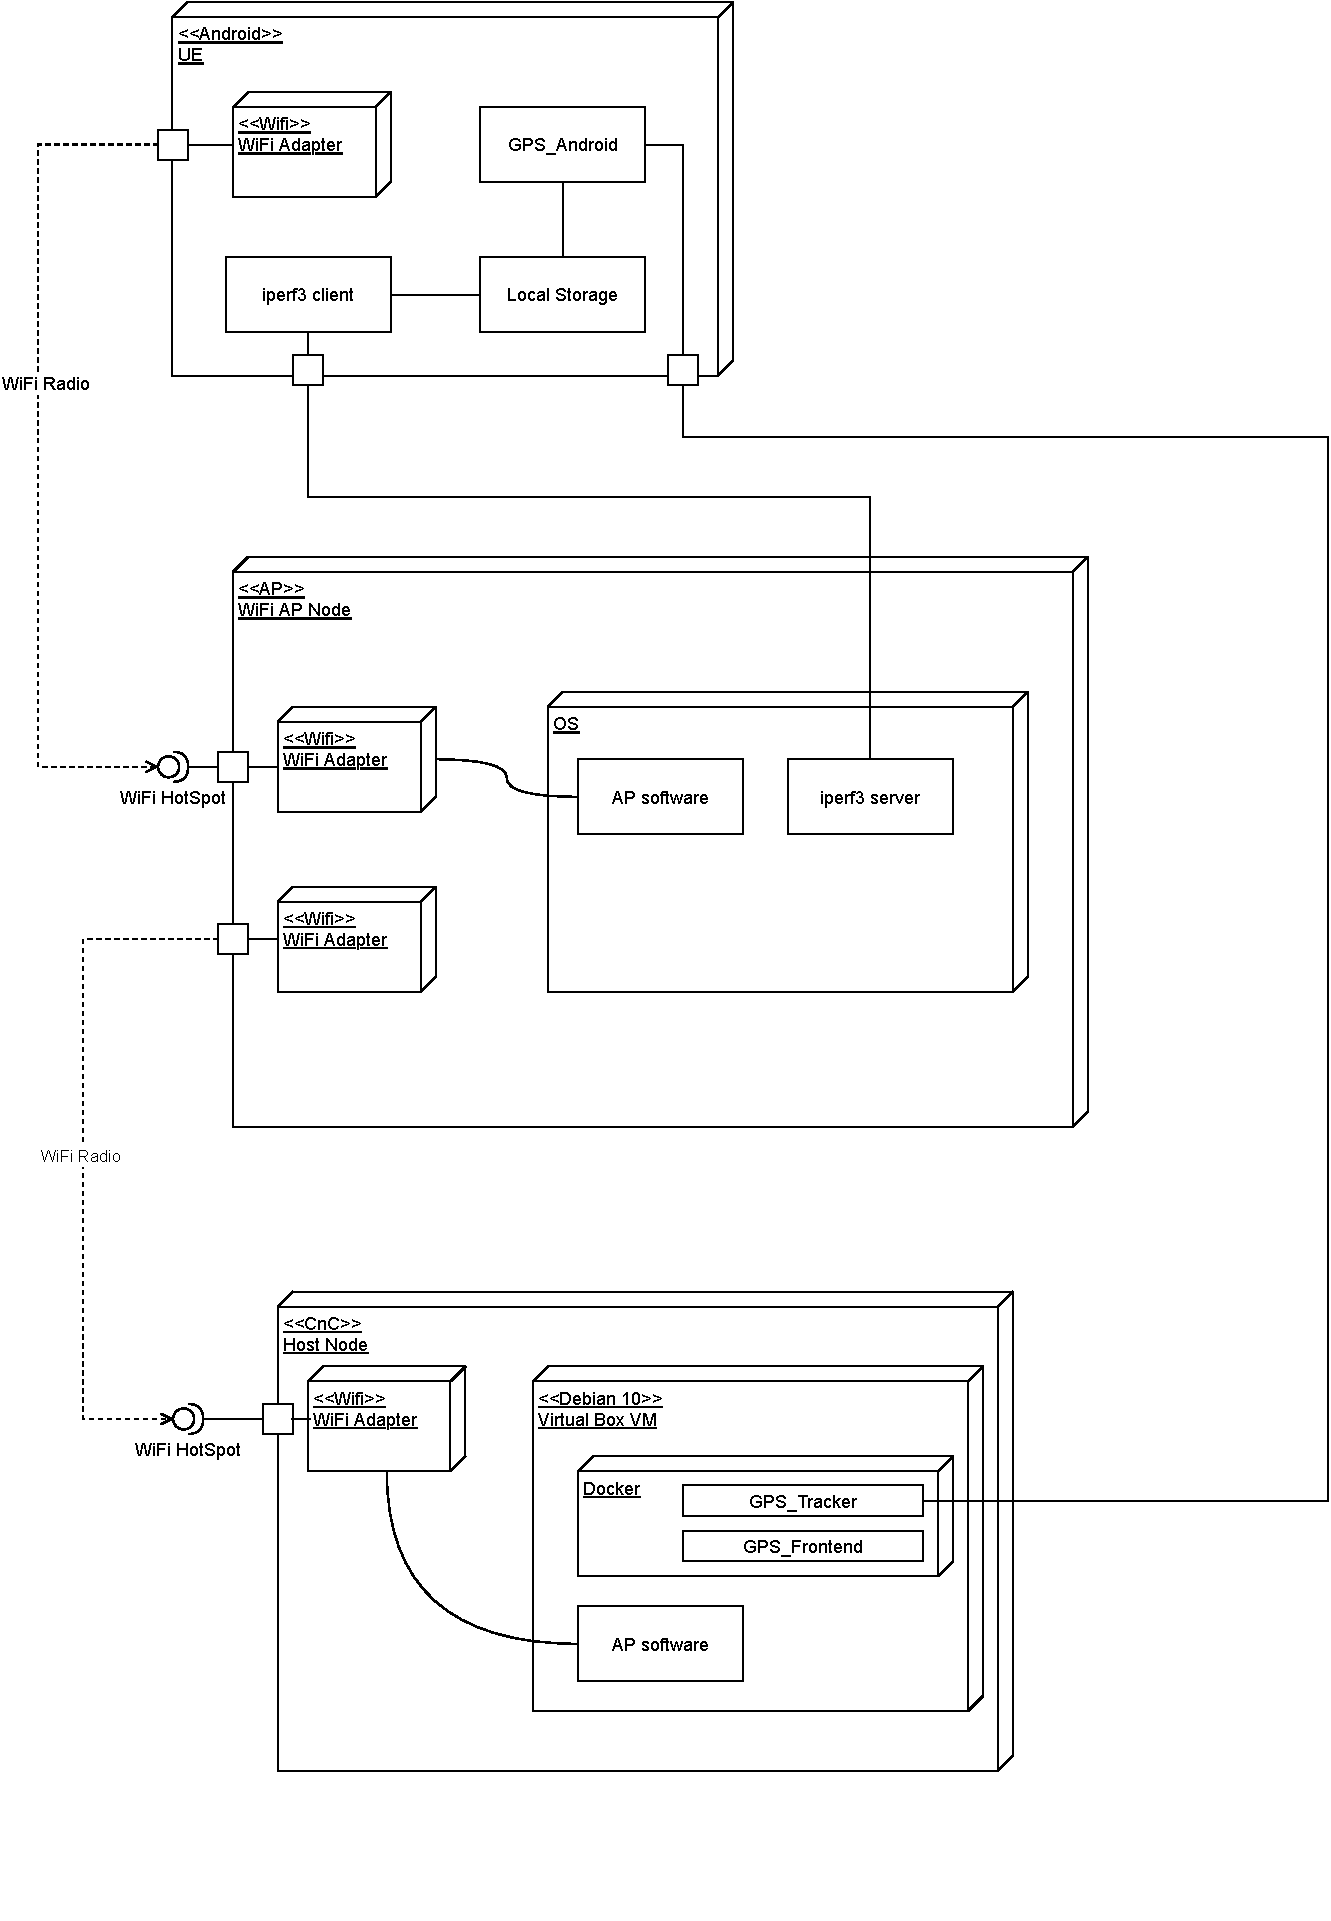
\includegraphics[width=0.7\linewidth, keepaspectratio]{images/Deployment Diagram-Deployment_Diagram.pdf}
	\caption{Deployment Diagram}
	\label{fig:deployment-diagram}
\end{figure}

We use virtual machines for running software components. It is possible to 
have performance decrease because of containers, however, more powerful
hardware resources compensates those possible consequences of additional 
run-time level. Hypervisor can pass-through access to physical equipment directly into guest operation system. To automate deployment of components, we use \gls{ansible}.

To start up a \gls{wifi} access point, it requires to have two packages in \acrshort{os}:

\begin{itemize}
\tightlist
\item
  \texttt{hostapd} - software to manage and run \gls{wifi} access points.
\item
  \texttt{dnsmasq} - \acrshort{dns}/\acrshort{dhcp} server, to provide an \acrshort{ip} address, routing
  and \acrshort{dns} information via \acrshort{dhcp} protocol.
\end{itemize}

\subsection{Network diagram}\label{network-diagram}


Figure \ref{fig:network-diagram} shows network configuration. The \glspl{ap} subnet has identical settings, they have an internal \gls{dhcp} server to provide dynamic addresses for connected \glspl{ue}. To prevent address collisions and to simplify routing, the \glspl{ap} perform masquerading (\acrshort{snat}/\acrshort{dnat}) on the output interface (connection to \gls{command_n_center}). Consequently, \gls{command_n_center} cannot access the \glspl{ue} directly, but \glspl{ue} will always reach \gls{command_n_center} because \acrshort{dhcp} server sets the default gateway IP address.

\gls{command_n_center} has another \acrshort{dhcp} server to set \glspl{ap} dynamic addresses. When \glspl{ap} connect to wireless point
``\textbf{cnc}'' they receive a dynamic IP address by \gls{command_n_center}.  Because network for \gls{command_n_center} is different from the internal networks of \gls{wifi} adapters in the \glspl{ap}, there is no network collision.

Finally, each connected \gls{ue} can access static \gls{command_n_center} address \texttt{192.168.20.1}
and local \acrshort{access_point} gateway \texttt{192.168.10.1}.


\begin{figure}[H]
	\centering
	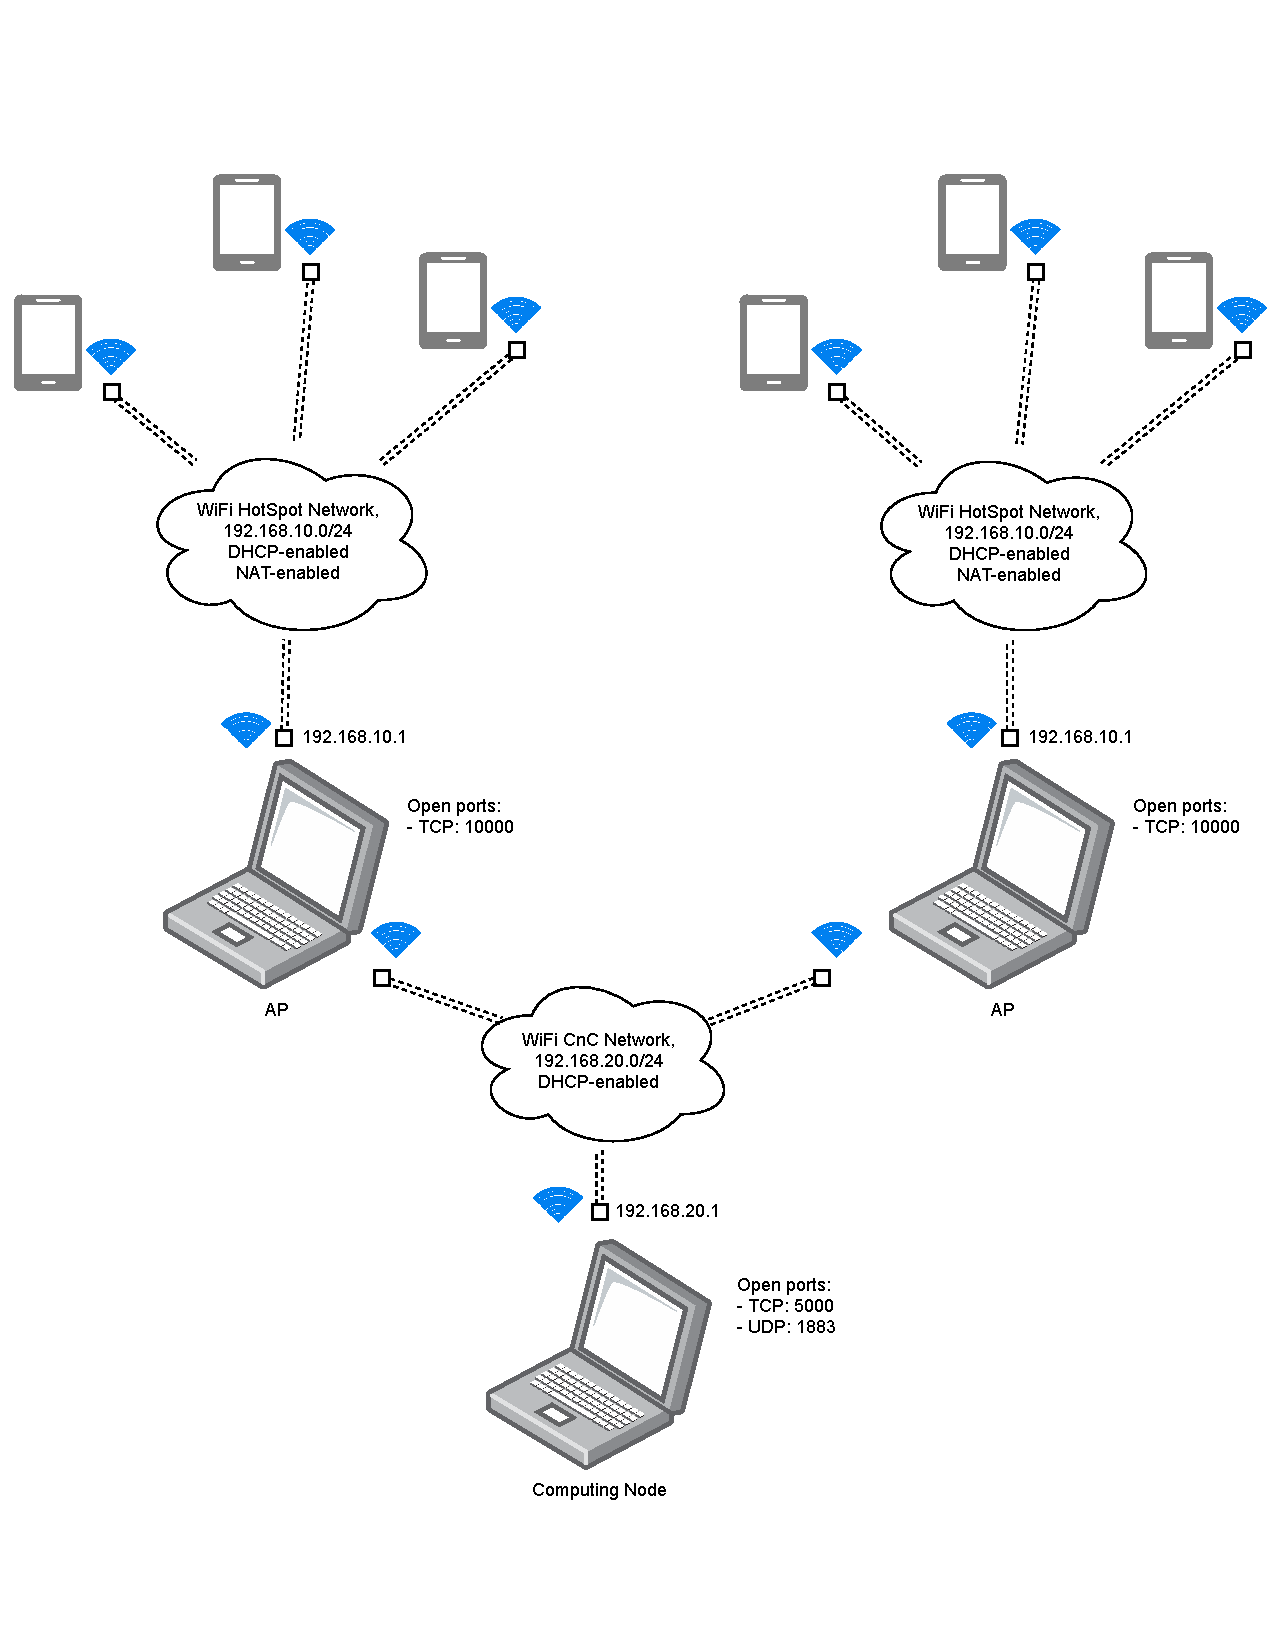
\includegraphics[width=\linewidth, keepaspectratio]{images/Deployment Diagram-Network_Diagram.pdf}
\caption{Network Configuration Diagram for experiment}
\label{fig:network-diagram}
\end{figure}

\subsection{Experiment steps}\label{experiment-steps}

The following steps will be executed for each described experimental
case:

\begin{longtable}[]{@{}lll@{}}
\caption{Steps for one experimental case.}\tabularnewline
\toprule
\begin{minipage}[b]{0.1\columnwidth}\raggedright
No
\end{minipage} & \begin{minipage}[b]{0.3\columnwidth}\raggedright
Step
\end{minipage} & \begin{minipage}[b]{0.5\columnwidth}\raggedright
Description
\end{minipage}\tabularnewline
\midrule
\endhead
\begin{minipage}[t]{0.1\columnwidth}\raggedright
1
\end{minipage} & \begin{minipage}[t]{0.3\columnwidth}\raggedright
Initialize network connectivity between \glspl{ap} and \gls{command_n_center}
\end{minipage} & \begin{minipage}[t]{0.50\columnwidth}\raggedright
Ensure using \acrshort{icmp}
protocol that all nodes are available in the network 
\end{minipage}\tabularnewline
\begin{minipage}[t]{0.1\columnwidth}\raggedright
2
\end{minipage} & \begin{minipage}[t]{0.3\columnwidth}\raggedright
Start up software
\end{minipage} & \begin{minipage}[t]{0.5\columnwidth}\raggedright
Startup \gls{gps_tracker}, \gls{gps_frontend}
\end{minipage}\tabularnewline
\begin{minipage}[t]{0.1\columnwidth}\raggedright
3
\end{minipage} & \begin{minipage}[t]{0.35\columnwidth}\raggedright
Place the \glspl{ap} and \glspl{ue} according to an experiment case
\end{minipage} & \begin{minipage}[t]{0.5\columnwidth}\raggedright
There are specific predefined positions for each element on the
experiment area.
\end{minipage}\tabularnewline
\begin{minipage}[t]{0.1\columnwidth}\raggedright
4
\end{minipage} & \begin{minipage}[t]{0.3\columnwidth}\raggedright
Measure \acrshort{rss}, Link quality for the initial layout
\end{minipage} & \begin{minipage}[t]{0.5\columnwidth}\raggedright
Measurements are done via \gls{gps_android} that sends the result to
\gls{gps_tracker}
\end{minipage}\tabularnewline
\begin{minipage}[t]{0.1\columnwidth}\raggedright
5
\end{minipage} & \begin{minipage}[t]{0.3\columnwidth}\raggedright
Run the \glspl{ap} location optimization for an algorithm in
\gls{gps_tracker}
\end{minipage} & \begin{minipage}[t]{0.5\columnwidth}\raggedright
Each method can give different results for
the same \gls{ue} input set.
\end{minipage}\tabularnewline
\begin{minipage}[t]{0.1\columnwidth}\raggedright
6
\end{minipage} & \begin{minipage}[t]{0.3\columnwidth}\raggedright
Move the \glspl{ap} to optimized positions.
\end{minipage} & \begin{minipage}[t]{0.5\columnwidth}\raggedright
It is expected that new coordinates for \glspl{ap} would increase our network
efficiency.
\end{minipage}\tabularnewline
\begin{minipage}[t]{0.1\columnwidth}\raggedright
7
\end{minipage} & \begin{minipage}[t]{0.3\columnwidth}\raggedright
Repeat \acrshort{rss} and link throughput measurements for the optimized \glspl{ap} positions
\end{minipage} & \begin{minipage}[t]{0.5\columnwidth}\raggedright
1-3 iteration per each case.
\end{minipage}\tabularnewline
\bottomrule
\end{longtable}
